\subsection{Slučaj upotrebe: Formiranje produkcionog tima}

\subsubsection*{Kratak opis}

Producent formira produkcioni tim za projekat animiranog filma tako što bira
zaposlene i dodeljuje im uloge na projektu. Kada tim ima sve obavezne uloge,
sistem angažuje članove na projektu i obaveštava ih.

\subsubsection*{Akteri}
\begin{itemize}
    \item \textbf{Producent} -- bira članove tima i njihove uloge na projektu.
\end{itemize}

\subsubsection*{Preduslovi}
\begin{itemize}
    \item Producent je prijavljen na sistem i odgovoran je za projekat.
    \item Projekat animiranog filma postoji u sistemu (slučaj upotrebe ,,Kreiranje filmskog projekta'').
    \item U sistemu su evidentirani zaposleni (slučaj upotrebe ,,Kreiranje zaposlenog i korisničkog naloga'').
\end{itemize}

\subsubsection*{Postuslovi}
\begin{itemize}
    \item Produkcioni tim projekta je sačuvan sa članovima i njihovim ulogama na projektu.
    \item Članovi tima su angažovani na projektu i obavešteni o tome.
\end{itemize}

\subsubsection*{Osnovni tok}
\begin{enumerate}
    \item Producent bira projekat i opciju ,,Formiraj produkcioni tim''.
    \item Sistem prikazuje trenutni sastav tima i listu zaposlenih koji mogu da se dodaju.
    \item Producent bira zaposlenog i njegovu ulogu na projektu.
    \item Sistem proverava da zaposleni nije već član tima i dodaje ga u tim. Koraci 3 i 4 se ponavljaju dok producent ne doda sve članove.
    \item Producent bira opciju ,,Potvrdi tim''.
    \item Sistem proverava da tim ima sve obavezne uloge.
    \item Sistem čuva tim, angažuje članove na projektu i šalje im obaveštenje.
    \item Sistem prikazuje sastav tima i poruku o uspešnom formiranju.
\end{enumerate}

\subsubsection*{Podtokovi: /}

\subsubsection*{Alternativni tokovi}

\paragraph*{A1: Zaposleni je već član tima}
\begin{itemize}
    \item Ovaj tok se dešava u koraku 4 osnovnog toka, ako je izabrani zaposleni već član tima tog projekta.
    \item Sistem obaveštava producenta da je zaposleni već u timu i prikazuje njegovu ulogu.
    \item Povratak na korak 3 osnovnog toka.
\end{itemize}

\paragraph*{A2: Nedostaju obavezne uloge}
\begin{itemize}
    \item Ovaj tok se dešava u koraku 6 osnovnog toka, ako tim nema sve obavezne uloge.
    \item Sistem prikazuje koje uloge nedostaju i ne dozvoljava formiranje tima.
    \item Producent dodaje članove koji nedostaju.
    \item Povratak na korak 3 osnovnog toka.
\end{itemize}

\subsubsection*{Specijalni zahtevi}
\begin{itemize}
    \item Tim projekta može da formira samo producent koji je odgovoran za taj projekat.
    \item Sistem beleži ko je i kada dodao svakog člana tima.
\end{itemize}

\subsubsection*{Dodatne informacije}
\begin{itemize}
    \item Podaci o članu tima (korak 3): zaposleni i njegova uloga na projektu.
    \item Lista zaposlenih (korak 2) sadrži aktivne zaposlene koji još nisu članovi tima i njihove uloge u sistemu.
    \item Zaposleni može da bude dodat samo u ulozi koja mu je dodeljena prilikom kreiranja naloga.
    \item Uloge na projektu: projektni menadžer, reditelj, scenarista, storyboarder, dizajner, animator, audio dizajner i montažer.
    \item Obavezne uloge (korak 6): bar jedan projektni menadžer i bar jedan reditelj.
    \item Zaposleni može da bude angažovan na više projekata, ali ima jednu ulogu u timu jednog projekta.
\end{itemize}


\begin{figure}[H]
	\centering
	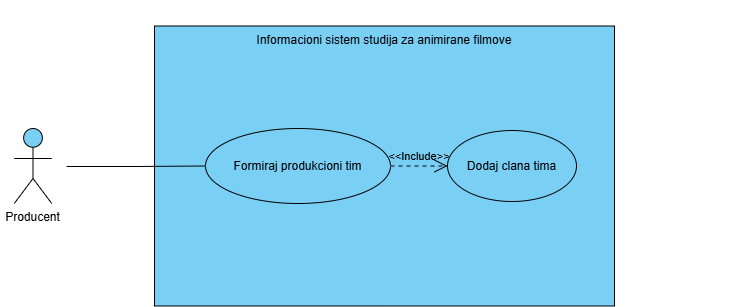
\includegraphics[width=\textwidth]{./dijagrami/dijagrami_slucajeva_upotrebe/formiranje_produkcionog_tima.png}
	\caption{Dijagram slučaja upotrebe ,,Formiranje produkcionog tima''}
 \end{figure}

\begin{figure}[H]
	\centering
	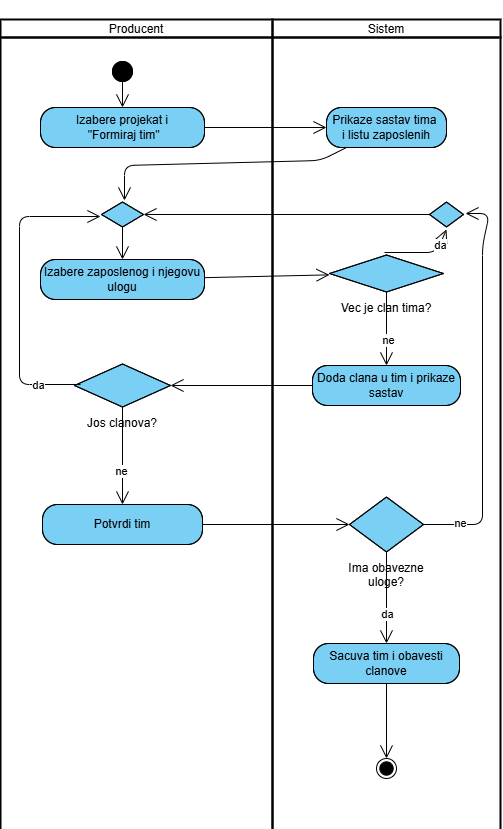
\includegraphics[width=\textwidth]{./dijagrami/dijagrami_aktivnosti/formiranje_produkcionog_tima.png}
	\caption{Dijagram aktivnosti ,,Formiranje produkcionog tima''}
 \end{figure}

\newpage
